\documentclass[UTF8]{scrartcl}

\usepackage{xeCJK}
\usepackage{graphicx}
\usepackage{subfigure}
\usepackage{indentfirst}
\setlength{\parindent}{2em}

%opening
\title{Aladdin工作原理}
\author{}

\begin{document}

\maketitle


\section{Introduction}

	Aladdin工作的核心原理是通过数据依赖图 (Data Dependency	Graph)表示加速器的行为。Graph中每个节点表示预定义的操作指令,边对应存储和寄存器依赖。硬件架构的各种设计调整均通过图结构的变换、节点属性的修改等方法体现。在此基础上,根据用户定义的硬件资源约束,使用图遍历算法(BFS)schedule 该graph,计算加速器的执行情况。最后,通过合适的binding策略将每个操作与实际的硬件资源对应起来,结合基本硬件资源的功耗模型,计算整个加速器的功耗。
	
				\begin{figure}[h]
					\centering
					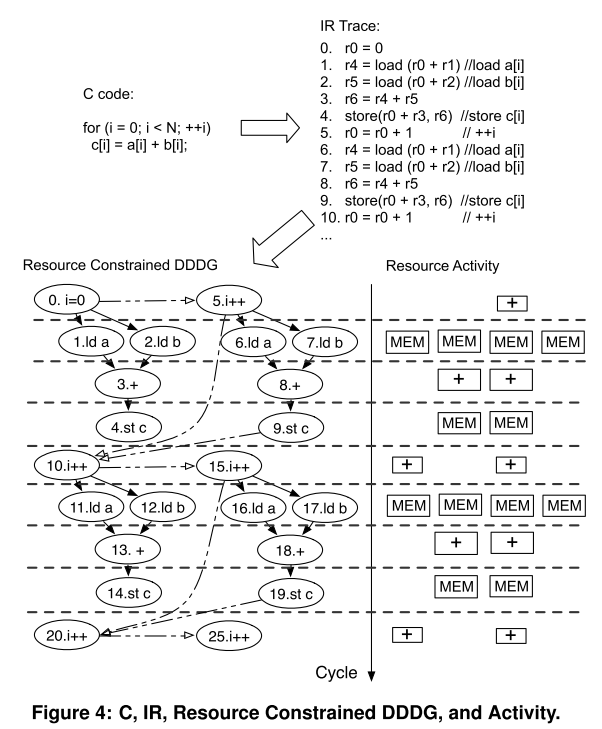
\includegraphics[width=4.00in,height=3.85in]{aladdin.png} 
					\caption{示意图}
					\label{fig1}
				\end{figure}
	
\section{Graph Construction}

	目标应用使用 c/c++描述,Aladdin依据代码执行的动态指令流构建动态数据依赖图。Aladdin使用LLVM IR,因为LLVM IR是机器无关的,能更好体现算法本身的行为,避免机器相关的指令如寄存器分配等的影响。图中的每个节点表示 LLVM IR 中的指令,而边表示节点之间的依赖包括存储/寄存器依赖等。
	
	
	首先使用 LLVM 的编译器前端 clang 将 c 代码翻译成 LLVM 的 IR 表示,然后通过在 IR 中添加指令获取函数(profiling functions)来定位和提取 trace。但这样修改后的 IR 无法真正在机器上运行,因此还需要一个just-in-time 编译器/解释器来执行修改后的 IR并生成运行时指令流。指令流中包括了指令的各项信息如指令ID、操作码、操作数、虚拟寄存器ID、存储地址(Load/store 指令)、代码块ID等。(	instruction IDs, opcodes, operands, virtual register IDs, memory addresses (for load/store instructions) and basic block IDs)

\section{Graph Transformation}

	\subsection{Graph Optimiztion}
	
		最初生成的 DDDG 还包含一些辅助节点和依赖边,与硬件行为无关。例如为了解决SSA 形式的变量赋值问题而添加的 PHI 节点和循环模块的索引变量依赖等。为了使	DDDG 主要表达加速器的硬件行为,无关节点会被删除或将latency设置为 0,无关的边会被移除,由此可获得完全体现实际计算行为的DDDG。
			
	\subsection{Hardware Transformation}
		
		
		
		\subsubsection{Array}
		
			代码中的array(数据)被映射为对应的存储资源,包括Memory(Scratchpad)和Register,访问不同的存储资源有不同的能耗和latency。
			
			如果array被映射为Memory,则在schedule时其load和store都需要作为一个独立node考虑,其访问有固定的latency(scratchpad访问地址是已知的),同时要考虑占用的端口资源(port)。用户可以设置Memory的尺寸、位宽、端口数、Partition策略等。
			
			当array被映射为Register时,处理情况与Memory类似,但其latency为0,即可以在同一周期中访问到其中数据。
		
		
		\subsubsection{Mem Access Optimizaton}
			
			根据指令trace中的地址和对memory的设置,指令流中的数据可以被映射到相应的地址中,并计算graph中的load/stroe操作的访存地址,根据这些信息可以对访存操作进行优化,移除冗余的laod/store指令,主要有以下三个方面:
			
			Shared load:如果两个load指令访问的是同一块地址且两个load间没有向该地址写入的store指令,那么load指令可以合并为一个。
			
			Store buffer:如果一个store节点是一个访问相同地址的load节点的直接前驱,则该load指令可以被移除,即使用数据buffer避免了写回再读出的浪费。
			
			Repeated store:如果两个store指令访问同一块地址且两者间没有数据依赖,则保留后一个store即可。
			
		\subsubsection{Loop}
		
			当循环中的计算没有Loop-Carried Dependeces时,通过将graph中循环索引变量的依赖、顺序执行时跳转指令的依赖移除,循环可以被展开,多个循环体内部计算可以并行进行。
		
		\subsubsection{Function}
			
			Graph中每个节点的属性中包含其属于的函数ID,在schedule和binding的时候可以依据此信息区分硬件中的不同模块。
					
		\subsubsection{Pipeline}
		
			Loop和funciton调用可以被pipelined执行,Pipeline的实现是通过将pre\_block的branch节点(表示该loop执行完成)与next\_block的执行节点之间的control edge(即pre中操作全部执行完才开始执行next) 移到 pre\_block的第一个非孤立节点和next\_block的执行节点之间(pre中的第一个操作执行完即开始执行next中的操作),由此两个Loop中的操作可以依次流水执行,每个node占用一个pipeline stage。
			
	
	
\section{Schedule}

	Schedule负责将Graph中的每个节点分配至相应的周期中,Aladdin中主要使用了两个策略,一个是ASAP(As-Soon-As-Possible),另一个是Resouce-Constrained Scheduling。
		
	依据ASAP策略,当Graph中一个节点的所有前驱节点(predecessors)执行完成时立即执行该节点。
		
	实际中还要考虑硬件资源的约束,即对ASAP的schedule结果再做修正。主要有以下几个方面的考虑:
		
	1.  时序约束:每个cycle schedule的节点的最大latency不能超过用户设定的cycle time,否则将该node schedule到下一个周期。
	
	2.  资源约束:每个scheduled node需要有可用的硬件资源。Aladdin在做schedule过程中会记录计算资源和存储资源的使用情况,当没有可用的计算单元或访存端口时,操作需要等待。

\section{Binding}
	
	Schedule将graph中的每个node分配至各个cycle,Binding则负责将每个操作与实际的硬件资源对应起来,主要考虑的是时间上的复用。由于复用需要占用MUX资源,Aladdin中对复杂的function unit如乘法器等进行复用,简单的unit如加法器、移位器等不复用。

\section{Dumpstats}
	
	通过schedule和binding,加速器执行中每个cycle的行为以及总的资源使用情况已知,结合每个操作对应的功耗可计算完整的功耗。功耗模型中考虑了不同latency下的动态功耗和静态功耗。
			

\end{document}
